\makeatletter\frontmatter@init\makeatother

\title{Gate-Sensing Anomalous Charge Pockets in the Semiconductor Qubit Environment}
\author{X. G. Croot}
\author{S. J. Pauka}
\author{M. C. Jarratt}
 \affiliation{ARC Centre of Excellence for Engineered Quantum Systems, School of Physics, The University of Sydney, Sydney, NSW 2006, Australia.}
\author{H. Lu}
\author{A. C. Gossard}
 \affiliation{Materials Department, University of California, Santa Barbara, California 93106, USA.}
\author{J. D. Watson}
 \affiliation{Department of Physics and Astronomy, Purdue University, West Lafayette, IN 47907, USA.}
 \affiliation{Birck Nanotechnology Center, Purdue University, West Lafayette, IN 47907, USA.}
\author{G. C. Gardner}
 \affiliation{Birck Nanotechnology Center, Purdue University, West Lafayette, IN 47907, USA.}
 \affiliation{Microsoft Quantum Purdue, Purdue University, West Lafayette, IN 47907, USA.}
\author{S. Fallahi}
 \affiliation{Department of Physics and Astronomy, Purdue University, West Lafayette, IN 47907, USA.}
 \affiliation{Birck Nanotechnology Center, Purdue University, West Lafayette, IN 47907, USA.}
\author{M. J. Manfra}
 \affiliation{Department of Physics and Astronomy, Purdue University, West Lafayette, IN 47907, USA.}
 \affiliation{Birck Nanotechnology Center, Purdue University, West Lafayette, IN 47907, USA.}
 \affiliation{Microsoft Quantum Purdue, Purdue University, West Lafayette, IN 47907, USA.}
 \affiliation{School of Materials Engineering and School of Electrical and Computer Engineering, Purdue University, West Lafayette, IN 47907, USA.}
\author{D. J. Reilly}
 \affiliation{ARC Centre of Excellence for Engineered Quantum Systems, School of Physics, The University of Sydney, Sydney, NSW 2006, Australia.}
 \affiliation{Microsoft Quantum Sydney, The University of Sydney, Sydney, NSW 2006, Australia.}

\makeatletter
\begingroup
\@author@finish
\frontmatter@author@produce@script
\endgroup
\makeatother

\begin{abstract}
Dispersive gate sensing (DGS) uses radio frequency (rf) reflectometry to locally probe the quantum capacitance of a gate electrode. Applying DGS to heterostructure-based qubit devices, we report the repeated observation of anomalous signals that we attribute to pockets of charge in the potential-landscape likely under, and surrounding, the surface gates that define quantum dot qubits. Interestingly, these charge pockets appear to evade detection with conventional charge sensors but manifest strongly in the response of the gate sensor. Configuring a quantum point contact (QPC) as a highly-localised heat source, we show how these charge pockets likely form close to the end of the gate electrodes, in close proximity to gate-defined qubits. The presence of uncontrolled charge may lead to offsets in gate-voltage, and further contribute to charge-noise that produces decoherence in semiconductor qubits.
\end{abstract}

\subsection{Introduction}

The on-chip resources needed to read out semiconductor qubits can be significantly lowered by using a single compact gate electrode as a detector \cite{Colless_PRL}. Configured to probe the local density of states by sensing the charge response to a small ac voltage, gate-based read-out has recently been shown to have sufficient sensitivity to enable the state of a qubit to be determined in a single shot \cite{Nnano_dzurak}. Despite recent advances \cite{fernando1,PhysRevApplied.10.014018,PhysRevX.8.041032}, it is not obvious that gate read-out can be deployed in all sensing regimes where single-electron transistors (SETs) or quantum point contacts (QPCs) have been used to detect the charge configuration of a nanoscale device \cite{Reilly:2007ig,Devoret_schoel}. In particular, since dispersive gate sensing (DGS) effectively detects a change in the local capacitance, its signal and noise spectrum can be different from those of conventional sensors that detect the total charge.

\begin{figure}
\includegraphics[width=0.75\linewidth]{figure1}
\caption[Several qubit devices used to examine the anomalous dispersive readout signal, and equivalent circuit schematic]{\label{fig:pock_fig1} (a-d) False-coloured micrographs of the four devices examined. Each device is fabricated from a unique GaAs/(Al,Ga)As heterostructure with mobilities of \SIlist[list-units=single]{3.9e6;0.44e6;2.4e6;4.8e6}{\square\centi\meter\per\volt\per\second}, densities \SIlist[list-units = single]{1.2e11;2.4e11;1.5e11;1.3e11}{\per\square\centi\meter}, and 2DEG depths of \SIlist{91;110;91;91}{\nano\meter} for device 1, 2, 3, and 4, respectively. White crossed boxes indicate ohmic contacts. Resonators, required for dispersive gate sensing, are indicated by the inductor symbols, with equivalent-circuit model shown in (e), including the parasitic capacitance $C_p$ and the classical gate capacitance $C_g$. (f) The reflection coefficient (S11) as a function of frequency of a typical resonator (attached to gate G1 of device 1) as the gate is biased from \SIrange{-290}{-990}{\mv}.}
\end{figure}

Here, we use DGS to investigate charge dynamics in the two-dimensional (2D) potential landscape of gate-defined qubit devices constructed from high-mobility heterostructure materials. Over the course of examining many different devices, we routinely observe reproducible but anomalous signals in the response of gate sensors as a function of the gate bias. Although not fully understood, we present data consistent with the interpretation that these anomalous signals originate from weakly bound pockets of charge that remain when the electron channel under or near a gate is only partially depleted. In this interpretation, large shallow quantum dots that are inadvertently trapped by inhomogeneities in the potential at low density \cite{PhysRevB.41.7929} undergo Coulomb blockade at low temperature. The rf voltage associated with the DGS technique can then induce tunnelling between trapped pockets of charge, leading to anomalous signals in the capacitive response of a gate. Surprisingly, these signals do not correlate with standard charge-detection measurements based on a QPC charge detector \cite{PhysRevLett.70.1311}. In what follows we propose an explanation to account for this discrepancy between DGS and charge sensing and present further evidence that these charge pockets are located reasonably close to the end of the gate electrodes.

The presence of such charge pockets has long been known, although directly probing them usually requires methods such as scanned-probe techniques \cite{Finkelstein90} that can, for instance, image electron-hole puddles \cite{PhysRevB.84.115442} at the surface of materials such as graphene \cite{Yacoby_scanned}. Puddles of charge have also been detected by measuring velocity shifts in the propagation of surface acoustic waves in low-density 2D systems \cite{TRACY2006150} or via the use of capacitive bridges \cite{Ashoori_science} and local electrometers \cite{Ilani1354}. Our use of gate sensing to probe the potential landscape extends this toolkit of techniques, opening the prospect of pinpointing unaccounted sources of noise and offset charge that limit the performance of qubits and read-out devices \cite{PhysRevLett.110.146804,Shulman202,Zoo_2Q}.

\subsection{Experimental Setup}
Turning to the details of our experiments, Fig.~\ref{fig:pock_fig1}~(a-d) show four separate GaAs/(Al,Ga)As devices with distinct gate patterns fabricated using electron-beam lithography and TiAu metallization for the gate electrodes. The growth of the heterostructure material spans separate molecular-beam epitaxy machines, and each device has been examined over multiple cooldowns and in different dilution refrigerators. The devices are also different in terms of their carrier density, mobility, and the depth of the two-dimensional electron gas (2DEG) from the surface (for details see the caption of Fig.~\ref{fig:pock_fig1}).  In the case of devices 3 and 4, the TiAu gate electrodes are separated from the GaAs surface by an \SI{8}{\nano\meter}insulating barrier of halnium oxide (HfO), deposited using atomic layer deposition. Devices 1 and 3 were cooled with positive bias \cite{PhysRevB.72.115331}. Despite all of these differences, anomalous oscillatory signals routinely appear in the response of the gate sensors, without any clear correlation to the device geometry or heterostructure material characteristics.

\begin{figure}
\includegraphics[width=0.65\linewidth]{figure2}
\caption[Signals of charge pockets under gates in quantum dot structures]{\label{fig:pock_fig2} (a) and (b) The complex, oscillatory pattern in the DGS response for device 1, as a function of gates G1 and G5, adjusting G3 by \SI{40}{\mv} between (a) and (b). This pattern does not resemble a typical DGS signal for a quantum dot.  (c), (d) The derivative of $V_{DGS}$ with respect to the gate bias, now as a function of G2 and G4. Active gates are held at constant potential and inactive gates at zero [see legend in (d)]. (e) A sketch illustrating our interpretation: charge pockets form underneath the gate when electrons are partially depleted, giving rise to Coulomb-blockade oscillations in the DGS readout signal.}
\end{figure}

Gates coloured orange in Fig.~\ref{fig:pock_fig1}~(a-d) are wire-bonded to radio-frequency (rf) $LC$ tank circuits to enable DGS using rf reflectometry \cite{Colless_PRL,doi:10.1063/1.4868107}. In this configuration, the capacitive component of the resonator comprises parasitic $C_p$, gate $C_g$, and quantum $C_q$ contributions, as shown in Fig.~\ref{fig:pock_fig1}~(e). A typical response of a resonator with frequency, shown in Fig.~\ref{fig:pock_fig1}~(f), depends strongly on the gate voltage, which alters the capacitance in the region of the gate electrode. With all other gates held at \SI{0}{\mv}, stepping gate G1 from low bias to a bias that fully depletes the 2DEG underneath the gate  shifts the resonant frequency as the reactance of the circuit changes. For subsequent figures the phase response is detected by mixing down the reflected rf carrier to baseband, yielding a voltage $V_{DGS}$ proportional to the change in resonator reactance at a fixed frequency.

Examining now the anomalous signals in the DGS response, Fig.~\ref{fig:pock_fig2}~presents representative data sets in which the response of the gate sensor (the red coloured gate in the Fig.~\ref{fig:pock_fig2}~insets) exhibits oscillatory patterns under various configurations of gate bias (see the caption for detailed explanation). Although the particular gate pattern was designed to produce quantum-dot qubits with tunnel coupling to the source-drain reservoirs, for the present study we intentionally do not bias the gates to values that would typically form a quantum dot in the centre region. Focusing on device 1, Fig.~\ref{fig:pock_fig2}~(a) shows the response of the gate sensor $V_{DGS}$ as a function of the gates G1 and G5, with the other gates held at constant bias. In this regime, the DGS response exhibits a complex pattern of lines that do not resemble the signal expected for an intentional quantum dot \cite{Colless_PRL}. Instead, the pattern of lines changes amplitude, period, and slope with the gate bias. A small variation in the bias of G3 dramatically alters the pattern [see Fig.~\ref{fig:pock_fig2}~(b)], providing the first clue that the signal originates from the electron gas, likely close to the end of the gates. To make it easier to see the fine details in these complex patterns, we plot the derivative of the sensing signal with respect to the gate voltage, as shown in Figs.~\ref{fig:pock_fig2}~(c) and (d), now as a function of G2 and G5.

\subsection{Discussion}
Breaking with our presentation of the data and moving to our interpretation, we suspect that these anomalous signals stem from charge transitions, not from an intentional quantum dot but from electrons tunnelling between disorder-induced charge pockets in the potential landscape. The sketch in Fig.~\ref{fig:pock_fig2}~2(e) illustrates this interpretation, showing how as the electron density is reduced by gate depletion, the homogeneous 2DEG breaks up into shallow puddles of charge, separated by tunnel barriers. The spatial distribution of such puddles is well understood \cite{PhysRevB.41.7929,Ilani1354} to reflect the configuration of partially ionized silicon donor sites in the Al(Ga,As), surface-charge arrangement, and crystal disorder at the heterostructure interface. Likely, as the gate bias is varied, the presence of these disorder-induced charge pockets leads to tunnelling transitions which can be detected with the dispersive gate sensing technique. Although not completely understood, we suggest that the curvature and changing slope of the lines relates to the complicated shape of the charge pocket and its response to fields from the gates, as well as the distance, orientation, and direction of tunnelling, relative to the gate sensor \cite{Ilani1354}.

\begin{figure}
\includegraphics[width=0.75\linewidth]{figure3}
\caption[Sensitivity of charge pockets to different gate configurations]{\label{fig:pock_fig3} (a) The DGS response for device 2, as a function of the bias on G3 and G4, with G1, G2 and G6 held at \SI{0}{\volt} to ensure that a quantum dot is not intentionally formed. (b) Close inspection of (a) reveals an avoided crossing. (c) The DGS signal as a function of G6 and G4. The response is insensitive to the bias applied to G6. (d), (e) For device 3, a comparison between the DGS response (d) when all gates are biased to low negative gate voltages and (e) at high negative gate voltages, where the oscillations are suppressed.}
\end{figure}

In what follows, we pursue this charge-pocket interpretation as an explanation for the complex patterns observed with gate sensing, gathering further evidence from measurements on additional devices.  Switching to device 2, for instance, we again observe oscillatory structure in the gate-sensor response, as shown in Fig.~\ref{fig:pock_fig3}~(a). In an effort to further pinpoint the source of this signal, we limit the gate bias to three gates, holding the other gates at zero to ensure that a quantum dot cannot be formed in the central region.  Nevertheless, even with three gates, close inspection of the data in Fig.~\ref{fig:pock_fig3}~(a) [see the enlarged region in Fig.~\ref{fig:pock_fig3}~(b)] reveals the presence of avoided crossings in the DGS signal and provides additional evidence that we are detecting interacting charge pockets in the potential landscape. Of interest, application of a voltage to the upper gate, G6, is seen to have no effect on the data, as shown in Fig.~\ref{fig:pock_fig3}~(c).

The strongest evidence that the anomalous patterns in the DGS response are associated with charge pockets is presented in Figs.~\ref{fig:pock_fig3}~(d) and (e), with data now taken on yet another device (device 3). Here, we compare the gate-sensor response, first with all other gates at low bias [Fig.~\ref{fig:pock_fig3}~(d)] and then with all other gates set to highly negative voltages [Fig.~\ref{fig:pock_fig3}~(e)], well past the typical bias required to deplete the electron gas. In the data taken in the high gate-bias regime, nearly all of the anomalous signals appear to vanish, again consistent with our interpretation that the signals arise from charge pockets that can be expelled with sufficient gate bias. Finally, we note that in the case of device 3, the surface gates are insulated from the GaAs by a thin layer of HfO. Despite the presence of the HfO, the oscillatory structure in the readout persists at low gate voltage, discounting explanations based on surface charge states or gate leakage, which would otherwise likely be modified by the addition of an insulating layer.

\begin{figure}
  \includegraphics[width=0.7\linewidth]{figure4}
  \caption[Comparison of QPC based charge sensing and dispersive gate sensing]{\label{fig:pock_fig4} A comparison of QPC-based charge sensing and DGS. (a) The differential conductance $dI/dV$ of a QPC formed with device 4, as a function of the gate and source-drain bias. (b) The corresponding response of the gate sensor for the same region of the gate and source-drain bias, $V_{\textrm{SD}}$. Note the appearance of the oscillatory structure around $V_{\textrm{SD}} = \SI{0}{\volt}$, which is absent in the transport measurement. (c) The data at  $V_{\textrm{SD}} = \SI{0}{\volt}$, showing a strong oscillatory response in DGS  (left axis) that does not correlate with features in the QPC transport (right axis), even near pinch-off where the QPC acts as a charge sensor.}
\end{figure}

Given our suspicion that the anomalous DGS signals arise from charge pockets under or near the gates, an obvious check is to look for comparable signals with conventional charge detectors such as an SET or QPC configured as a sensor, by monitoring its conductance close to pinch-off. Measurements with device 4 enable such a direct comparison, as shown in Fig.~\ref{fig:pock_fig4}. Here, we form a QPC by pinching off the electron gas between gates G2 and G3 and measuring the transport current between ohmic contacts, as shown in Fig.~\ref{fig:pock_fig4}~(a). Although this QPC does not exhibit clean quantized conductance plateaus, it pinches off steeply near zero bias to make a good charge sensor. We then compare the transport response of the QPC to the signal from the DGS sensor [Fig.~\ref{fig:pock_fig4}~(b)], both measured as a function of source-drain bias  $V_{\textrm{SD}}$. Clear in the DGS response is the presence of an oscillatory pattern around $V_{\textrm{SD}}$ = \SI{0}{\volt}, typical of the signal that we interpret as tunnelling between charge pockets in Coulomb blockade. Interestingly, this oscillatory signal begins to weaken as the QPC opens up (the lighter, diamond-like features near G2 $\sim \SI{-400}{\mv}$ relate to the DGS detecting the first QPC subband edge \cite{MC_paper}). Comparing the response of the two detectors at zero bias, Fig.~\ref{fig:pock_fig4}~(c) displays a strong oscillatory signal in the DGS response (blue) that extends well past the gate bias at which the QPC pinches-off. In contrast, the QPC transport signal (red) does not show any discernible features that correspond to the oscillatory structure in the DGS signal.

We suggest two explanations to account for the discrepancy between the signals from the two detectors. First, the location of the charge pockets is likely under, or very close to, the gate, since this is where the electrons are depleted by the gate bias. In this picture, a charge pocket could be far from the QPC and strongly screened by the gate metal to the extent that it is undetectable by the QPC sensor. Alternatively, if the pocket is under the gate it is always closely coupled to the gate and can alter its quantum capacitance. In fact, screening by the gate metal constitutes the DGS signal. Second, we note that in the case of DGS the oscillating rf voltage on the gate induces the tunnelling transitions, which are detected synchronously, i.e., in relation to the phase of the rf signal, whereas the QPC charge sensor makes a time-average measurement of the induced charge.

\begin{figure}
  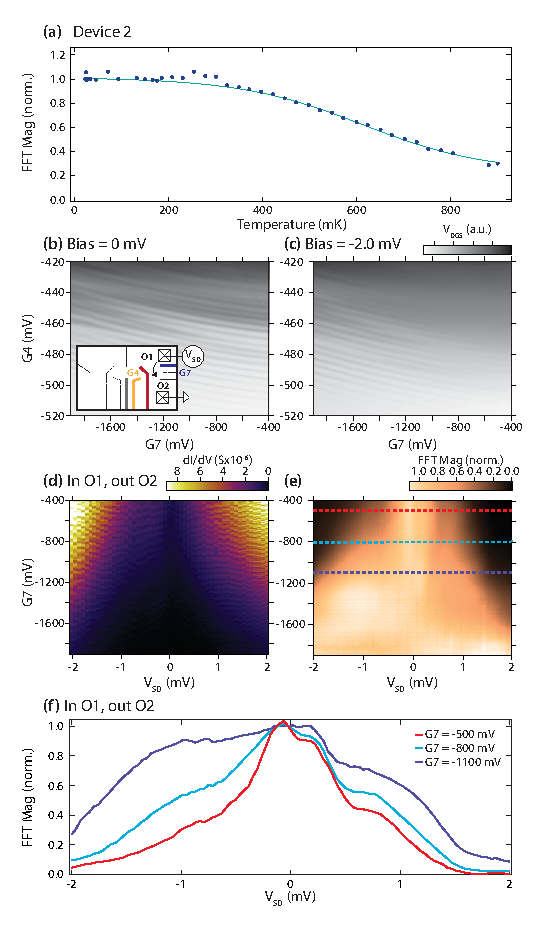
\includegraphics[width=0.65\linewidth]{figure5}
  \caption[The effect of bias and heating on the visibility of the anomalous sensing signal]{\label{fig:pock_fig5} (a) The temperature dependence of the DGS oscillations, as quantified by their Fourier amplitude, normalised with respect to their amplitude at a base temperature of approximately \SI{20}{\mk}. The line is a guide to the eye. (b) The DGS response as a function of G7 and G4, without a source-drain bias across the QPC. (c) DGS oscillations with a QPC bias of $V_{\textrm{SD}}$ = - 2.0 mV. (d) The differential conductance of the QPC as a function of the source-drain bias $V_{\textrm{SD}}$. (e) The amplitude of the DGS oscillations, quantified as the magnitude of their Fourier component, as a function of the gate bias G7 and $V_{\textrm{SD}}$. (f) Horizontal one-dimensional line cuts of the data in (e) at positions indicated by dashed lines.}
\end{figure}

We next examine the temperature dependence of the patterns seen in the DGS response, and in keeping with our interpretation that they arise from charge pockets, extract their charging energy. Taking device 2 as an example, Fig.~\ref{fig:pock_fig5}~(a) shows the amplitude of the anomalous DGS oscillations [measured as the magnitude of their fast Fourier transform (FFT)] as a function of the cryostat temperature. Raising the temperature  above $T \sim \SI{300}{\mk}$ rapidly suppresses the oscillations in the DGS signal, presumably as the thermal energy becomes comparable to the charging energy of the pocket, that is, on the order of a few tens of microelectronvolts, an order of magnitude smaller than the typical charging energies measured for intentional, gate-defined quantum dots used as a qubits \cite{Hanson:2007eg}. Such a small charging energy is consistent with a large capacitance between the charge pocket and the gate, as could be expected if the pocket is underneath or very closely coupled to the gate.

Finally, in an effort to better pinpoint the location of the charge pockets we make use of a QPC as a highly local source of joule heating. By controlling the bias across the QPC, this approach allows a very small amount of heat to be generated at the micron-scale region surrounding the QPC, as opposed to elevating the temperature of the whole chip, essentially creating a local temperature gradient. Biasing gates G7 and G5 to configure a QPC, we control the dc voltage across ohmic contacts O1 and O2 and perform DGS readout from gate G5, as shown in Figs.~\ref{fig:pock_fig5}~(b) and (c). At low gate bias, with the QPC open and low resistance, the presence of current between O1 and O2 has little effect on the oscillations in the DGS signal. When the QPC is partially closed, however, the presence of a source-drain bias, $V_{\textrm{SD}}$, leads to suppression in the oscillatory pattern measured by the gate sensor, as indicated by comparing Fig.~\ref{fig:pock_fig5}~(b) ($V_{\textrm{SD}} = \SI{0}{\mv}$) to Fig.~\ref{fig:pock_fig5}~(c) ($V_{\textrm{SD}} = \SI{-2}{\mv}$). The oscillations are restored when the QPC is fully pinched off and the current drops to zero.

Investigating further, we make a more detailed examination of this effect by first measuring the QPC differential conductance, as shown in Fig.~\ref{fig:pock_fig5}~(d). As the QPC is nearly pinched off, appreciable conductance only appears at high $V_{\textrm{SD}}$. Next, we quantify the amplitude of the DGS oscillations by taking their FFT magnitude as a function of $V_{\textrm{SD}}$ and the gate bias, G7, as shown on the intensity axis in Fig.~\ref{fig:pock_fig5}~(e) and as 1D line cuts in Fig.~\ref{fig:pock_fig5}~(f). In this way, we are making use of the anomalous DGS signal from the pockets as a highly local thermometer. We can calibrate this (Coulomb-blockade) thermometer using the data in Fig.~\ref{fig:pock_fig5}~(a), which gives the FFT magnitude of the oscillations as a function of the cryostat temperature. With this calibration in hand, we determine that the presence of a modest source-drain bias across the QPC, say \SI{0.5}{\mv}, dissipates only picowatts of power, but surprisingly heats the charge pockets to a temperature of the order of approximately \SI{700}{\mk}. Given that the cryostat has a cooling power of hundreds of microwatts at this temperature, and given crude estimates for the thermal conductivity of the chip, we conclude that the QPC creates a hot spot that returns to the bulk equilibrium temperature over a scale of the order of the electron scattering length $l_\phi$. This reasoning, although somewhat tentative, is again consistent with our interpretation that the location of the charge pockets is within a few microns of the QPC hot spot, likely not at the very tip of the gates but, rather, under the wider sections of the gates as they taper out and are partially depleted.

\subsection{Conclusion}
Throughout this paper, we present data consistent with our interpretation that electron tunnelling between unintentional charge pockets leads to oscillatory signals in the dispersive response of gate sensors. Summarising, this evidence includes the following: the sensitivity of the oscillatory patterns to the bias of nearby gates (Fig.~\ref{fig:pock_fig2}); the presence of avoided crossings (Fig.~\ref{fig:pock_fig3}~(b)); and the suppression of signals when gates are fully depleted (Fig.~\ref{fig:pock_fig3}~(d)). Carrying this argument further, the data in Fig.~\ref{fig:pock_fig4}~show that these signals are not detectable with a QPC charge sensor, presumably because screening from the gate metal makes them difficult to detect using standard charge sensing --- in contrast to DGS, where the pockets contribute directly to the quantum capacitance of the gate. Finally,  the data in Fig.~\ref{fig:pock_fig5}~suggest that the charge pockets are reasonably localized to the vicinity of the QPC, and, given their small charging energy, it is likely that such pockets correspond to shallow micron-scale quantum dots that form directly under the gates as the electron gas is partially depleted. Counting the number of Coulomb-blockade oscillations, we estimate these pockets contain tens of electrons or more.

Drawing attention to the possibility that these shallow pockets may be perturbed by proximal QPC transport and considering that qubits are operated by rf gate pulses or microwaves, it is likely that their presence can lead to charge fluctuations during qubit readout and control. The extent to which these pockets can be alleviated via the use of bipolar induced-electron device structures \cite{PhysRevLett.89.246801,PhysRevApplied.6.054013} is an open direction for mitigating noise and offset charges in semiconductor qubits.

\subsubsection{Acknowledgments}
This research was supported by the Microsoft Corporation (Quantum Sydney), the US Army Research Office grant W911NF-12-1-0354, and the Australian Research Council Centre of Excellence for Engineered Quantum Systems (EQUS, CE170100009). We thank A.C. Mahoney for technical assistance and discussions, and acknowledge the contributions of J.I. Colless, for the fabrication of device 2, and J.M. Hornibrook, for the development of the readout multiplexing chips. We acknowledge the use of the Australian National Fabrication Facility for device lithography.
